\section{Transposition des graphes en cartographie}
%intro

\subsection{Spécification des attributs topographiques des sommets}
La spécification des attributs des sommet se fait par un tableau de données placé en paramètre de la fonction \textit{vertex\_attr()}. Ce tableau doit remplir deux conditions  : il ne peut pas y avoir de doublon parmi  les noms des sommets, et,  le tableau doit recenser entièrement et exclusivement  les sommets du graphe.
Pour cela,  nous créons un nouveau tableau de données, \textit{df\_nodes}, sur la base des noms de sommets récupérés par la fonction \textit{V(g)\$name}, puis nous remplissons de valeurs \textit{NA}.

Nous revenons un peu en arrière dans le script d'extraction des relations pour rajouter une ligne de code qui enregistrera, lors de la scission de l'énoncé de la rente en deux parties, le débiteur  ainsi que le numéro de la rente  dans un tableau de données \textit{df\_débiteur\_rente}. 
\begin{figure}
    \centering
    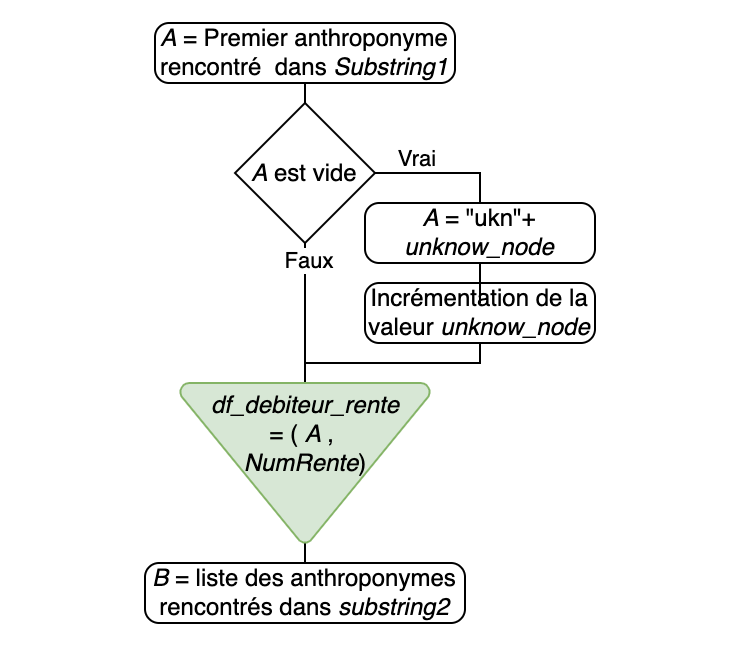
\includegraphics[scale=0.75]{3.Results/Img/extrac_rel_mod.png}
    \caption{Modification du script d'extraction des relations en vue de récupérer les informations relatives aux débiteurs}
    \label{fig:mod_rel}
\end{figure}

Tel qu'illustrer par la figure \ref{fig:from_main}, le tableau de données \textit{df\_debiteur\_rente} nouvellement créé, va servir à récupérer les informations topographiques relatives à chaque sommets en servant de lien entre le tableau de données des noeuds, contenant uniquement les noms de sommets à ce moment,  et le tableau de données principal.

\begin{figure}
    \centering
    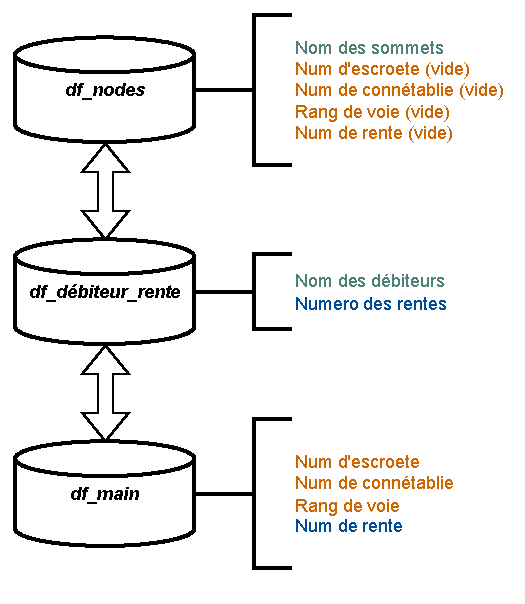
\includegraphics[scale=0.75]{3.Results/Img/rel-from_main.drawio.pdf}
    \caption{Tableau de données des attributs des sommets}
    \label{fig:from_main}
\end{figure}

Le tableau de donnée des noeuds est encore fort lacunaire à ce stade car il ne contient que les données relatives aux débiteurs des rentes. Celles relatives aux sommets voisins et n'étant pas débiteur de Jean de France sont encore manquantes. Comme expliqué dans le chapitre \textit{Méthodes}, nous ne disposons pas des informations exactes concernant ces sommets, nous ne pouvons que supposer, avec prudence, de celles-ci. Afin d'enrichir le tableau,  la règle définie dans ce même chapitre est appliquée.

Après ce processus, nous pouvons constater que le tableau de données \textit{df\_nodes} a été fortement enrichi, comme le montre le tableau \ref{tab:df_nodes}.
\begin{table}
    \centering
    \begin{tabular}{|c|c|c|}
    \hline  \textbf{Numéro d'escroete} & \textbf{Numéro de connétablie} & \textbf{Rang de voie} \\
    \hline
    \hline 24 & 31 & 195 \\
    \hline 4,26\% & 5,51\%  & 34,63\% \\
    \hline
    \end{tabular}
    \caption{Valeurs manquantes dans tableau de données des sommets}
    \label{tab:df_nodes}
\end{table}\footnote{De nombreuses connétablies ne possédant pas deux rangs de voie distincts, il est à noter que les chiffres de la colonne << Rang de voie >> ne sont pas représentatifs des lacunes du tableaux de données }

\subsection{Importation des fonds de cartes}
L'import des fonds de cartes sur \textit{R}  se fait par la fonction \textit{get\_map()} de la bibliothèque \textit{ggmap}. 
Celle-ci prend comme paramètres un vecteur contenant la position géographique de deux points permettant de découper un rectangle sur le planisphère, la source d'import des images, ainsi que le type de carte voulu.
Par défaut, cette fonction se connecte à l'\textit{API} de \textit{Google Maps}. Malheureusement, depuis 2018,  l'usage de l'\textit{API} requiert une clé  et les requêtes sont facturées. Par conséquent, il faut changer la source d'import des fonds de cartes par \textit{OpenStreetView} ou \textit{Stamen maps}, des alternatives libre d'accès. Cependant, ceci nous confronte à un nouveau problème : ces  catalogues de cartes sont pas aussi riches que celui de \textit{Google Maps} et il nous faut choisir entre une  concéder à une résolution médiocre ou  avoir des tuiles manquantes. Finalement, en changeant le type de carte en <<  watercolor  >> un compromis relativement acceptable à été trouvé.

\begin{figure}
    \centering
    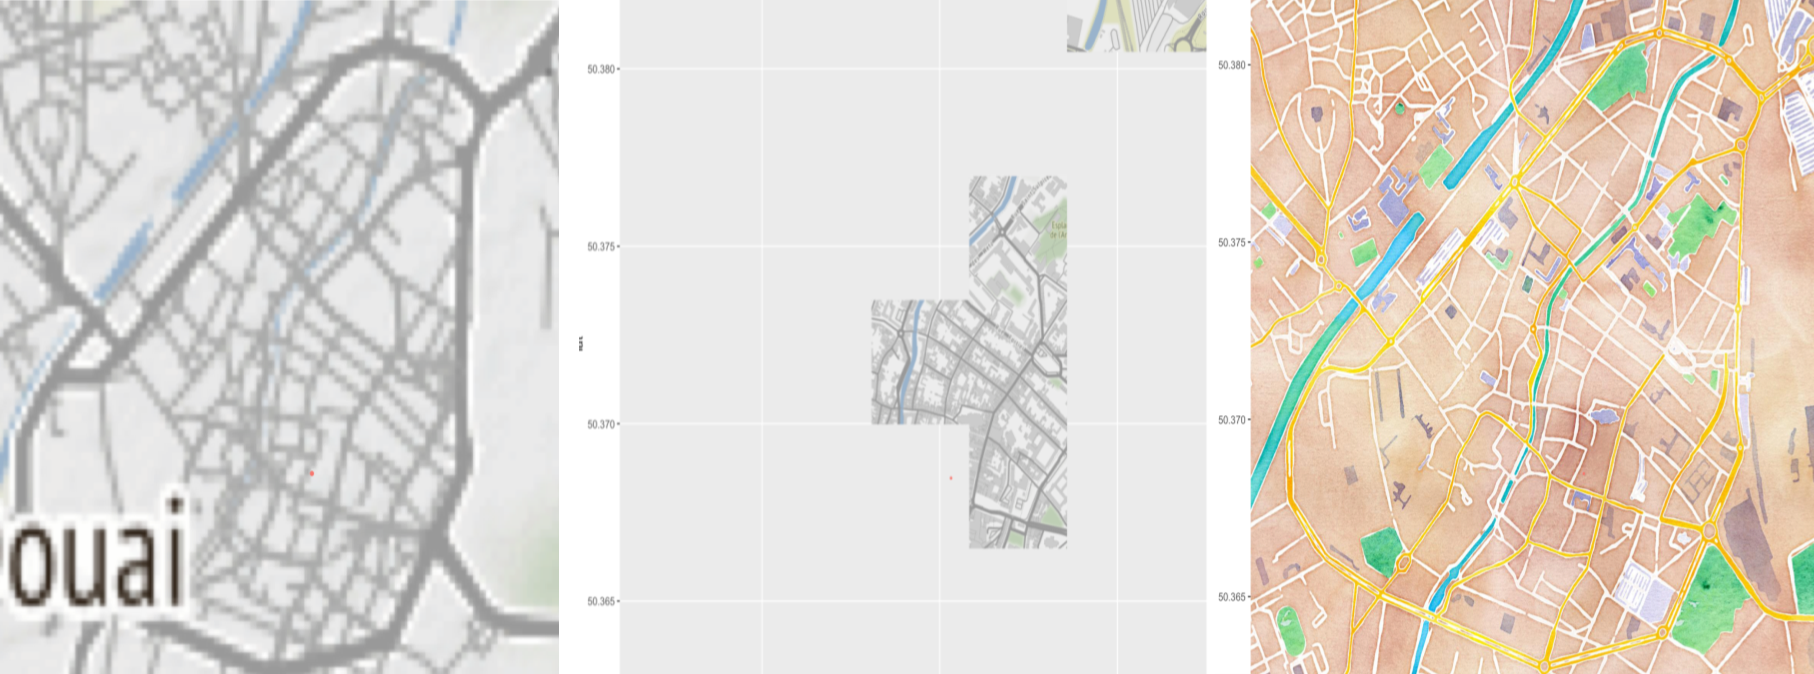
\includegraphics[scale=0.4]{3.Results/Img/maps.png}
    \caption{Différents fonds de carte}
    \label{fig:maps}
\end{figure}

\subsection{Repères topographiques}
L'étape suivante consiste à replacer des repères sur la carte importée par la fonction \textit{ggmap()}.
Aidé par une série d'ouvrages et de rapports de fouilles archéologiques \footfullcite{colin_decouvrez_2001,salamagne_construire_2020,liegeard_recherche_1859,demolon_les_1979,demolon_service_1999,demolon_douai_1990} qui se sont avéré particulièrement précieux dans cette tâche, l'étape suivante consiste à replacer des éléments topographiques du Douai du XIIIe siècle sur une carte du Douai actuel. Ceci dans le but d'en retrouver les coordonnées géographiques et de s'en servir comme <<  ancrage  >> pour le graphe des rentes.

On commence donc par chercher l'emplacement des connétablies dont il est fait mention dans le rentier. Rares sont les rues et places ayant gardé leur nom d'origine. Pour cause, au Moyen Âge, le nom des connétablies provient généralement des corps de métiers qu'elles concentrent (rue des foulons), des paroisses proches (Rue Saint Pierre),  du lieu auquel elles mènent (Porte d'Arras), ou d'un élément topographique particulier(Outre le pont Sainte Margrite). Or la physionomie de la ville  a fort changée  au cours du temps (de nouveaux corps de métiers se sont implantés, des éléments topographiques ont disparûts, des paroisses ont été démantelées, etc.) et avec elle, le nom des rues.

\subsubsection{Connétablies}
Si l'aspect pragmatique des toponymes du Moyen Âge facilite grandement la recherche de correspondances avec le présent, il peut cependant se montrer traître  et créer des confusions. D'une part, parce que certaines connétablies ont plusieurs toponymes différents, par exemple : la porte Saint-Jacques qui est nommée ainsi par rapport à l'ancienne église Saint-Jacques qui fut à proximité de la porte, sur l'actuelle place Carnot, est également appelée << porte de la Nuevile >> car elle donne accès à cette partie de la ville. D'autre part, car ces toponymes peuvent faire référence à des éléments topographiques n'existant plus à notre époque. Les fossets inondés qui longeaient les enceintes ou les multiples bras de la Scarpe qui traversaient la ville peuvent être cités pour l'exemple. Il en ressort des noms de connétablies tels que << Ou pont >> qui, au premier abord, semble donc n'avoir aucun sens.

A ces difficultés il faut rajouter celle que de nombreuses rues ont, depuis le XIIIe siècle, été fusionnées (la rue de la trinité  avec la ruelle Dame Ydain le Cousturière,  pour former la rue François Cuvelle), prolongées (la rue du Kiosque\footnote{Anciennement  rue \textit{Pute i muce}}, ou totalement supprimées (\textit{rue fait-en paille}).

Le recoupement manuel des sources permis de composer un tableau de correspondance entre entre les noms de connétablies et les adresses des rues et places actuelles.
Sur les 75 connétablies recensées dans le registre, 11 n'ont pas pu être retrouvées, principalement pour les raisons sus nommées. 

Une fois le tableau de correspondance importé, la méthode \textit{geocode()} de la bibliothèque \textit{tidygeocoder} va récupérer les coordonnées géographiques des adresses correspondantes aux anciennes connétablies et accoler les données de latitude et longitude  au tableau de correspondance.
Dans un même temps, un nouveau tableau de données (\textit{df\_conn\_nodes}) est créé à partir du tableau de données principal, en sélectionnant les noms et numéros de connétablies et d'escroetes correspondantes. En opérant une jointure interne sur la colonne du numéro de connétablie, les deux tableaux sont fusionnés ensemble et chaque connétablie est alors reliée à ses informations géographiques (latitude, longitude) et topographiques (numéro et nom d'escroete). Finalement, la fonction \textit{geom\_node\_point()} prend les informations géographiques en paramètre pour replacer les connétablies sur la carté générée par \textit{ggmap}. 


\subsubsection{Portes et enceintes}
Ensuite le placement des enceintes, et surtout des portes,  nous offre un second ensemble de repère intéressant.
Sur la totalité des portes et tours qui fusent jadis, il n'en reste malheureusement que trois :  la porte d'Arras, la porte de Valenciennes\footnote{Anciennement appelée << porte de Nostre Dame >>, en relation avec l'église du même nom située en deça, ou  << porte de Vakeresse >> qui se traduirait par << porte des vaches >>\parencite{demolon_service_1999} et ferait probablement référence au marché des bestiaux qui se tenait sur la place du Barlet}, et la tour des Dames.  Il est à noter aussi que la morphologie exacte des remparts du XIIIe siècle, avant leur fortification en pierre, est relativement mal connue \parencite{demolon_douai_1990}. 

A travers les sources,  les emplacements de neuf portes de la première enceinte et de sept pour la seconde  enceinte ont pu être identifiés. 
Leurs coordonnées  ont été prises manuellement depuis \textit{Google maps} et placées dans un tableau de données. Les portes  sont affichés sur la carte de la même de manière que les connétablies. Un tracé rejoins celles-ci afin de représenter approximativement les murs d'enceintes de la ville. La totalité des portes n'étant pas représentée sur la carte (par manque d'informations), le tracé  des murs est incorrect sur certaines sections (principalement  la partie Nord-Est, entre la porte de Morel et  la porte de Valenciennes.
Toute foi, le résultat obtenu (figure \ref{fig:mapName}) ne semble pas trop éloigné de ce qu'il peut être observé sur carte présenté dans le chapitre \textit{Introduction} (figure \ref{fig:planDouaiIntro}).

\subsubsection{Points de correspondances}
Le replacement approximatif des connétablies et des enceintes offre  un ensemble de points de repères précieux, mais afin de lier le graphe des rentes à des point précis de la carte, il reste encore à trouver des correspondances exactes entre des éléments cités dans les énoncés des rentes du registre et la ville actuelle. Ainsi, l'étude des lieux suivants semble être commencement adéquat.

\begin{itemize}
\item	Le tenement des Malades	cité dans les rentes 	7.1, 14.8 et 95.3
\item	Le tenement des Charteriers	cité dans les rentes 	15.9 et 104.1.
\item	La porte Frères Menus	citée dans la rente 	24.12.
\item	Le fosset de la ville	cité dans la rente 	43.2.
\item	La jonction avec la rue de Canteleu	citée dans la rente 	119.1.
\item	La porte de la Nuevile 	citée dans la rente	128.4.
\item	L'ospital des Wés	cité dans les rentes 	153.6 et 206.5.
\item	La jonction avec la ruiele du Més	citée dans les rentes 	159.3 et 160.4.
\item   La porte des Saint-Nichaolaï citée  dans la rente 162.6.
\item   Le moulin de Robert d'Estrees cité dans la rente 162.6.
\item	La jonction avec la rue Pute i muce	citée dans la rente	178.3.
\item	L'ospital Wérin Mulet cité dans la rente	262.1.
\end{itemize}


\subsubsection{Tenement des Charteriers}
Le tenement des Charteriers\footnote{Qu'on le retrouve également sous l'écriture << Carteriers >> et << Chatriers> >} correspond à l'ospital des Charteriers --- qui selon  selon l'expression, fut << fondé d'anchienneté et hors de mémoire d'homme >>\footfullcite[p.73]{dubois-druelle_douai_1845} --- se situait à l'emplacement de l'actuel square Jemappe entre la rue de Valenciennes. On peut l'apercevoir sur le plan de Braun (figure \ref{fig:demolon99}, numéro: 5) ainsi que la restitution de l'ancien parcellerai de la rue François Cuvelle (figure \ref{fig:françoiscuvelle}). 

\subsubsection{Tenement des Malades}
Le tenement des Malades, que l'on retrouve aussi sous les appellations  de << Hôpital des Malades >>, <<  Maison des Malades >> ou encore << Maison des Lépreux >> est un établissement destiné aux lépreux provenant de la bourgeoisie Douaisienne. Il est évoqué à de nombreuses reprises et à travers différentes sources, mais sans jamais qu'il soit fait mention de son emplacement précis. Il semblerait par ailleurs qu'il ait existé simultanément plusieurs << Maisons des malades >>. Au mieux une une source en dit : << établie dans les faubourgs de Douai >>\footfullcite[p.73]{dubois-druelle_douai_1845}, sans plus de précision.
D'après ce qui peut être déduit des énoncés des rentes 7.1 et 15.9,  le tenement des malades devrait s'être situé non loin de l'ospital des Charteriers, juste à  l'entrée de la ville  << En le Grant rue >>.  Cependant certaine source le suppose plutôt à l'extérieurs de la porte de Valenciennes \parencite{brassart_notes_1842}
L'emplacement du tenement des Malades reste donc trop incertain pour servir de point de concordance.

\subsubsection{Porte des Frères Menus}
La portes des Frères Menus, ou Frères Mineurs, n'est pas une l'une des portes d'enceinte mais l'entrée de la ruelle Frères Menus, menant à leur couvent \parencite{duthilloeul_douai_1864}. Celui-ci était juxtaposé à l'ancien fosset de la première enceinte, comme on peut le voir sur la figure \ref{fig:demolon99}, et doit correspondre à l'actuelle place De Gaule. 

\subsubsection{La porte de la Nuevile et de Saint-Nicholaï}
Il s'agit de deux des anciennes portes de la première enceinte menant respectivement à l'escroete de la Nuevile et aux quartiers sud  de la ville. La porte de Saint-Nicholaï prend sont nom de l'église voisine, quant à la porte de Nuevile elle tire son nom dz la Nuevile, anciennement faubourg, et ensuite englobé par la seconde enceinte. Cette dernière est également appelé << Porte Saint-Jakeme >> ou << porte Saint-Jacques >> en référence à l'église  qui se tenait sur l'actuelle place Carnot.

\subsubsection{L'ospital des Wès}
L'ospital des wés, dit aussi << Du Saint Esprit >> fondé par Gervais de le Ville en 1245  était une maison béguinale. l'établissement sayait contre la porte des Wés, au coin de la rue du béguinage \parencite{brassart_notes_1842}.

\subsubsection{Le moulin de Robert d'Estrees}
selon l'énonce de la rente 162.6, le moulin de Robert d'Estrees est censé se trouver à proximité de la porte Saint-Nicholaï, la rue Foucques étant à cette époque traverser par un bras du petit bail de la Scarpe. Plusieurs sources mentionnent une roue près de  l'abreuvoir de Sint-Nicolas, le  << miredol >> \parencite{lohrmann_entre_1984,brassart_memoire_1862,colin_decouvrez_2001}, mais aucune n'en donne la localisation précise.

\subsubsection{L'ospital Wérin Mulet}
L'hôpital connu, aussi sous les noms de << Saint-Marguerite >> ou des << femmes gisantes >> fut fondé par Wérin mulet en 1274. Il fût érigé dans ce qui était la grande rue St-Piere, correspondant aujourd'hui à la rue Léon Ganbetta, et siégerait, d'après un annuaire  de 1808  au numéro 14 \parencite{brassart_notes_1842}.

\begin{figure}
    \centering
    \includegraphics[scale=0.80]{3.Results/Img/françoisCuvelle.png}
    \caption{Topographie médiévale des environs de la rue François Cuvelle sur le plan de Braun de 1656, copie d’un document de 1627\footfullcite[p.11]{demolon_service_1999}.}
    \label{fig:françoiscuvelle}
\end{figure}

\begin{figure}
    \centering
    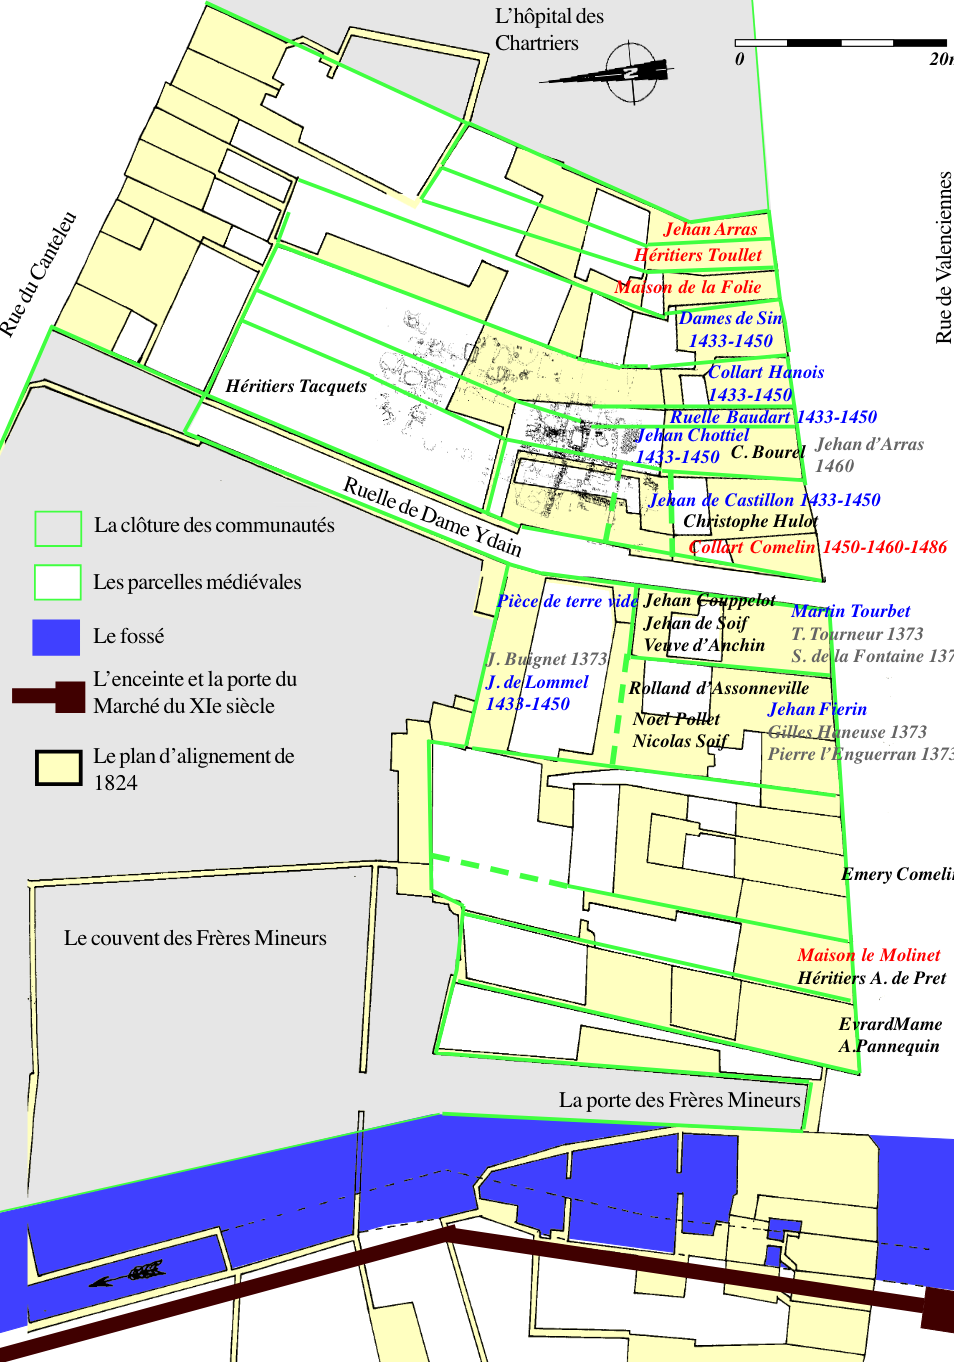
\includegraphics[scale=0.80]{3.Results/Img/demolon99.png}
    \caption{Proposition de restitution du parcellaire médiéval et fin médiéval établie à l’aide des archives et des résultats des fouilles\footfullcite[p.26]{demolon_service_1999}.}
    \label{fig:demolon99}
\end{figure}

Tous les points de repères évoqués plus n'ont pas été détaillés. Pour cause, les emplacements de jonctions entres rues  sont implicite à eux même, si tant est  que la situation des rues  est elle-même connue. 
Quant au fosset de la ville, que l'ont peut observer au numéro 7 de la figure \ref{fig:demolon99}, si son emplacement approximatif est connu, il semble compliqué de lui donner des coordonnées géographiques précises. 

Au terme de cette brève étude, nous pouvons dégager une liste de quelques points de concordances dont les coordonnées géographique sont récupérées depuis \textbf{Google maps} puis importées dans \textit{Rstudio} sous la forme d'un tableau de données. A l'instar des portes d'enceintes, ces points sont placés sur la carte via la fonction \textit{geom\_node\_point()}.

Cette opération rompt malheureusement en grande partie avec l'idéal d'automatisation du processus, mais au vu de la complexité de celle-ci, aucune alternative à cette partie ne parait envisageable dans le cadre de ce travail.

\section{Superposition des graphes sur le fond de carte}
Le système développé avait pour objectif de produire une cartographie de la ville de Douai et d'y placer les graphes obtenus à partir de la fouille de texte automatisée du censier de Jean de France. Pour arriver à cette fin, deux éléments étaient nécessaires : la production d'un fond de carte avec un système de références géographiques et la production de graphes modélisant les liens de mitoyenneté entre les entités. Les deux ont pu être obtenus séparément : le fond de carte par les fonctions de la bibliothèque \textit{ggmap} et les graphes par celles de la bibliothèque \textit{ggraph}. Cependant, et malgré les différents outils essayés (\textit{Gephi}, \textit{tkplot}, \textit{ggmap}, \textit{igraph}, \textit{ggraph}), il semble impossible de coupler les deux objets produits ensemble, comme deux couches d'un même objet graphique. Thomas Lin Pedersen, développeur travaillant sur les bibliothèques du \textit{tidyverse} dont sont issues les deux bibliothèques sus nommées, confirme dans un poste sur la platforme github qu'il s'agit d'une fonctionnalité qu'il souhaite implanter dans le futur, mais qu'elle n'est, à priori, pas prévue avant la prochaine version de \textit{ggplot2}. Le commentaire de Thomas Lin Pedersen est daté du 04 mars 2017, mais aucune information plus récente n'a été communiqué sur le sujet.

\begin{displayquote}
    << I absolutely want a way to combine ggraph with maps. My current sentiment is that I'll wait for the native sf support that will arrive in the next version of ggplot2 rather than get tangled in with another extension >> 
    \footfullcite[url : https://github.com/thomasp85/ggraph/issues/24 - consulté le : 02/08/2022 à 19:24]{noauthor_combine_nodate} \footnote{ << Je veux absolument un moyen de combiner ggraph et maps. Mon sentiment actuel est que j'attendrai le support natif sf qui arrivera dans la prochaine version de ggplot2 plutôt que d'y mêler une autre extension}
\end{displayquote} 
\vspace{0,5cm}
Face à cette limite, les cartes produites se concentreront uniquement sur les données dont des coordonnées géographiques peuvent être obtenues, de manière automatiques ou manuelles, ou sur des données agrégées.

\section{Cartographies produites}
Avant toute chose, il est à garder à l'esprit que les cartes présentées ne constituent qu'une proposition pouvant contenir d'éventuelles erreurs ou imprécisions. Les informations ayant servies à leurs élaboration proviennent soit d'algorithmes de traitement automatisé, soit du recoupement d'un nombre limité de sources qui, parfois, comportent elles-même des imprécisions ou ne semblent pas correspondre à ce qui est décrit dans le registre de rente.
De plus, il est à noter aussi que le fond de carte provient d'une version contemporaine du planisphère. Il n'est donc pas exactement en phase avec les éléments décrits au travers des cartes et certains aspects topographiques du XIIIe siècle , tels que les fossets ou le bras de la Scarpes,  n'y sont pas représentés. 

En outre, les cartes présentées ne respectent pas toutes les règles de la représentation cartographique. Ceci est principalement le fait de l'outil utilisé pour les produire et cet aspect sera expliqué plus en profondeur dans le
chapitre \textit{Discutions}.
\subsection{Cartes des noms de portes et des points de repères}
Cette première carte (figure \ref{fig:mapName}), assez simple, est une projection des connétablies dont la correspondance avec les lieux actuels a pu être établie. On y indique le nom des portes ainsi que les points de repère cité dans le registre qui auraient du servir à << ancrer >> le graphe sur la carte.
\begin{figure}
    \centering
    \includegraphics[scale = 0.80]{3.Results/Img/mapName.pdf}
    \caption{Carte indiquant les noms des portes et des points de repères de Douai au XIIIe siècle}
    \label{fig:mapName}
\end{figure}
\subsection{Carte des emplacements des connétablies}
La seconde carte (figure \ref{fig:mapConnetablie}), comme la première,  est une projection des connétablies dont la correspondance avec les lieux actuels a pu être établie. Cette fois  ce sont les numéros de connétablies qui y sont indiqués. Dans l'idéal, ces deux première cartes n'en n'auraient formées qu'une seule et les nom des connétablies auraient été affiché au lieu de leurs numéros. Malheureusement, la résolution et le format des fond de cartes utilisés nous contraint quant à la taille de la carte. Et se faisant, les noms se seraient chevauchés, rendant la carte illisible.
\begin{figure}
    \centering
    \includegraphics[scale = 0.80]{3.Results/Img/mapConnetablie.pdf}
    \caption{Carte indiquant les numéros des connétablies citées dans le rentier de Jean de Rente}
    \label{fig:mapConnetablie}
\end{figure}

\subsection{Carte de la densité des rentes }
La carte suivante (figure \ref{fig:mapNbRente}) indique le nombre de rentes acquises par Jean de France dans les différentes connétablies. Ces quantités sont représentées par un  nombre ainsi que par la taille  d'une aire centrée sur l'indicateur de la connétablie.
\begin{figure}
    \centering
    \includegraphics[scale = 0.80]{3.Results/Img/MapNbRente.pdf}
    \caption{Carte indiquant le nombre de rentes  de Jean de France dans chaque connétablie}
    \label{fig:mapNbRente}
\end{figure}


\subsection{Cartes des escroetes}
La carte  des escroetes (figure \ref{fig:mapEscroete})  utilise la fonction \textit{geom\_mark\_hull()} de la bibliothèque \textit{ggforce} pour circonscrire les connétablies dans des aires d'après les informations topographique issues de l'extraction des rentes. L'objectif est d'observer l'emplacement approximative des escroetes citées dans le registre de rentes.

\begin{figure}
    \centering
    \includegraphics[scale = 0.80]{3.Results/Img/mapEscroete.pdf}
    \caption{Carte représentant approximativement les escroetes citées dans le rentier de Jean de France}
    \label{fig:mapEscroete}
\end{figure}

\subsection{Cartes des anthroponymes}
La carte  des anthroponymes (figure \ref{fig:mapAnthro}) indique la localisation des habitants au niveau des connétablies.
Une jointure entre le tableau de données df\_nodes, produit à partir du graphes des rentes et le tableau de données df\_conn\_nodes  a permis de faire correspondre les différents anthroponymes aux connétablies marquées sur les cartes précédentes. Il était assez prévisible que l'affichage d'autant de noms  sur une carte aux dimensions restreintes rende celle-ci peu lisible. Afin de palier à cela,  on préférera n'en faire ressortir qu'une sélection en v avec . La figure \ref{fig:mapFocus} en est un exemple avec la célèbre famille Boinebroke.

\begin{figure}
    \centering
    \includegraphics[scale = 0.80]{3.Results/Img/Rplot_anthro.pdf}
    \caption{Carte indiquant les anthroponymes cités dans le rentier de Jean de France}
    \label{fig:mapAnthro}
\end{figure}

\begin{figure}
    \centering
    \includegraphics[scale = 0.80]{3.Results/Img/Rplot_focus.pdf}
    \caption{Carte centrée sur la Famille Boinebroke}
    \label{fig:mapFocus}
\end{figure}

\subsection{Carte des rentes}
Finalement, la dernière carte affiche les numéros des rentes consignées dans le registre en fonction des connétablies.
\begin{figure}
    \centering
    \includegraphics[scale = 0.80]{3.Results/Img/Rplot_rentes.pdf}
    \caption{Carte indiquant les rentes consignées dans le rentier de Jean de France}
    \label{fig:mapRente}
\end{figure}

\section{Observations}
Les cartes produites permettent d'observer des informations  qui se recoupent avec d'autres sources. Pour reprendre celle centrée sur la famille Boinebroke\footnote{c.f. figure \ref{fig:mapFocus}},  on peut y observer que des propriétés possédées par Jehan Boinebroke se situent dans la connétablie n°35, soit la rue des Foulons.
Une information que l'on retrouve également dans différentes sources :
\begin{displayquote}
    << Sire Jehan possède dans la ville basse de Douai, sur la rive droite de la Scarpe, une habitation personnelle, dont il a fait le siège administratif de sa florissante entreprise de drap. C'est là qu'il installe son bureau, qu'il traite ses affaires, qu'il bâtit un dépôt dans lequel s'empilent laines brutes et teintures et des étoffes prêtes à la vente et aux expéditions. Derrière sa maison, au-delà d'une dérivation de la rivière, s'élève son atelier de teinturerie, et plus bas, dans la même rue des Foulons, l'atelier de tendage. >> 
    \footfullcite[p.37]{thibault_histoirehistoires_1997}
\end{displayquote} 

La carte du nombre de rentes par connétablie\footnote{c.f. figure \ref{fig:mapNbRente}} permet également d'appuyer les propos de G. Espinas lorsqu'il nous dit : 
\begin{displayquote}
    << Enfin, les propriétés arrentées se trouvent toutes situées sur la rive droite de la Scarpe et, pour la plupart, dans le voisinage de la demeure même du patricien [...] >> 
    \footfullcite[p.107]{espinas_les_1933} 
\end{displayquote} 
Demeure que G. Espinas suggère sise << \textit{deheurs le porte dou Markiet} >> \parencite{espinas_les_1933}. Ce qui correspond à la connétablie 2°bis et à l'actuelle rue de Valenciennes où, en effet, on peut remarquer sur la carte, que la  majorité de ses rentes sont situées sur la rive Est, et sont concentrées autour de la connétablie 2°bis.

Ce ne sont ici que deux exemples d'observations qui peuvent être fait. L'intérêt final de ce système et des cartographies produites seront discutés plus amplement dans le chapitre suivant.


